%========================================================================================
% TU Dortmund, Informatik Lehrstuhl VII
%========================================================================================
\chapter{Physik}
\label{Kapitel 4}

Um die Bewegungen des Ball möglichst realistisch und nachvollziehbar zu realisieren und somit dem Nutzer ein echtes Spielgefühl zu vermitteln, müssen einige physikalische Eigenschaften der "{}echten Welt"{} ins Spiel implementiert werden. In diesem Fall heißt es, dass die Reflexionen eines Balls auf einer Oberfläche richtig berechnet werden müssen. Dementsprechend müssen auch Kollisionsabfragen dafür realisiert werden. Des Weiteren soll die Bewegung des Balls innerhalb der Box korrekt berechnet werden sowie ein Gravitationsfaktor die Fallgeschwindigkeit beeinflussen können.

Da im Programm in jedem Durchlauf der Hauptschleife zuerst die Bewegungen und dann die Kollisionen bzw. die Reflexionen berechnet werden, wird auch in diesem Kapitel diese Reihenfolge beibehalten.
\section{Bewegungen}
\label{Kapitel_4_-_Unterkapitel_1}
Die verschiedenen physikalische Eigenschaften des Balls werden in der Klasse BallPhysics verwaltet. Dazu gehören: Masse, Kraft, Gravitation und Geschwindigkeit.
%====================Kraft wird nicht benutzt!!================
%===================Wahrscheinlich noch ändern=================
Bei jedem Tick wird die Update-Methode des Balls aufgerufen, die wiederum für die Positionsbestimmung zunächst die Update-Methode der Klasse Ballphysics aufruft, die die aktuelle Geschwindigkeit berechnet. Da die Geschwindkeit als 3-dimensioneller Vektor gespeichert wird, ergibt sich daraus auch immer die Richtung in die der Ball sich bewegt. Dabei wird zunächst die Beschleunigung des Balls, die durch die Masse und die Gravitationskraft beeinflusst wird, berechnet und schließlich auf den Geschwindigkeitsvekor addiert.
 \begin{equation}
	    \label{beschleunigung}
	    Beschleunigung = (\frac{1}{Masse} + Gravitation) * t 
    \end{equation}
Mithilfe des Geschwindigkeitsvektor lässt sich dann die nächste Position des Balls bestimmen:
\begin{equation}
	    \label{beschleunigung}
	   \mathbf{x}_{t+1} = \mathbf{x}_{t} + \mathbf{v}\Delta t 
    \end{equation}
Schließlich werden dann basierend auf der neuen Position die Rendering-Informationen aktualisert. 


\section{Reflexion}
\label{Kapitel_4_-_Unterkapitel_2}

Nachdem die Positionen aktualisert wurden, wird geprüft, ob an den neuen Positionen Kollisionen aufgetreten sind. Dies geschieht in der {\texttt{CollisionResolver}}-Klasse. Die Funktion {\texttt{resolveCollisions(Ball* ball, Racket* racket, Box* box)}} wird von der Hauptschleife aus aufgerufen und überprüft zuerst die Kollision des Balls mit der Box bzw. mit den 6 Ebenen der Box und dann die Kollision mit dem Schläger.
Die Ebenen werden in einer Hesseschen Normalform ähnlichen Darstellung gespeichert, sodass der Abstand des Balls zu einer Ebene leicht berechnet werden kann.

\begin{figure}[h]
    \subfigure[]
          {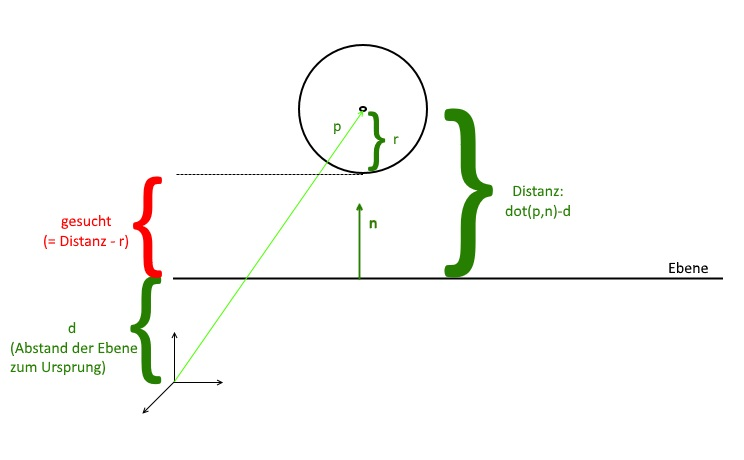
\includegraphics[scale=0.8]{bilder/collision}\label{fig_testbild_a}
    }
    \caption{Übersicht der Kollisionsüberprüfung}
        \label{fig_testbild}
\end{figure} 

Da die Hessesche Normalform wie folgt aussieht,$ E: \vec x \cdot \vec n  = d $, und d der Abstand zum Ursprung ist, lässt sich die Formel umformen zu $ E: \vec x \cdot \vec n  - d = 0$. Diese Formel ist erfüllt wenn $\vec x$ auf der Ebene liegt. Ersetzt man also 0 durch eine Variable $c$, kann der Abstand von Punkt $\vec x$ zur Ebene genau ermittelt werden. In unserem Fall erlauben wir auch negative Abstände; negative Abstände entstehen dann durch Ballpositionen, die hinter der Ebene liegen (entgegen der Richtung des Normalvektors).
Der Abstand des Ballmittelpunkts zur Ebene ist also $c = \vec p\cdot \vec n - d $. Somit lässt sich eine Kollision feststellen, wenn der Abstand zur Ebene kleiner als der Radius des Balls ist.

Damit der Ball bei zu hohen Geschwindigkeiten nicht hinter die Ebene gelangt und die Kollision nicht erkannt wird, wurde eine Kollisionsüberprüfung implementiert, die genau dies verhindern soll (nach \cite{migGom:1999}). Denn bei dieser Methode wird der Ball auf eine Position vor der Ebene zurückgesetzt, falls er tatsächlich hinter die Ebene gelangt. Das Prinzip ist wie folgt:

Es werden immer die letzten beiden Positionen des Balls gespeichert ($C_0$, $C_1$) und die Distanzen zu beiden Zeitpunkten nach schon beschriebener Weise berechnet ($d_0, d_1$).
Befindet sich $C_0$ vor der Ebene und $C_1$ hinter der Ebene bzw. ist $d_0$ positiv und $d_1$ negativ, so wird die neue Position des Balls zwischen diesen beiden Punkten interpoliert (s. Formel \ref{interpolEquation1} und \ref{interpolEquation2}). 
\begin{equation}	
\label{interpolEquation1}
	u = \frac{d_0 - r}{d_0 - d_1}
\end{equation}
\begin{equation}	
\label{interpolEquation2}
	C_{neu} = (1-u)C_0 + uC_1
\end{equation}

\begin{figure}[h]
   \begin{center}
       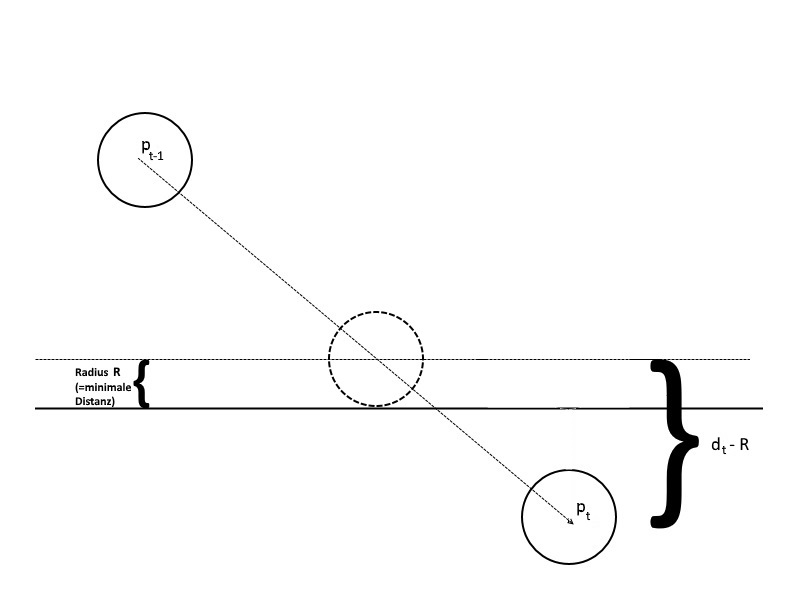
\includegraphics[scale=0.5]{bilder/interpolation}\label{fig_interpolation}
   \end{center}
    
    \caption{Interpolation der Ballposition bei vollständigem Durchstoßen der Ebene}
        \label{fig_interpol}
\end{figure} 

Ist der Ball nicht vollständig hinter die Ebene geflogen - d.h. es gilt $d_1<0$ und $|d_1|<R $ - dann wird der Ball um $R - |d_1|$ in Richtung des Normalenvektors der Ebene verschoben.

Die Kollisionserkennung mit dem Schläger verläuft nach ähnlichem Schema ab. Auch die Fläche des Schlägers wird als Ebene gespeichert. Es muss also auch nur der Abstand zu Ebene berechnet werden und mit dm Radius des Balls verglichen werden. Ist der Abstand kleiner gleich dem Radius, dann kollidiert der Ball mit dem Schläger. Jedoch ist Der Schläger keine unendlich große Fläche wie die  Boxwände, sondern ist auf eine bestimmte Kreisfläche begrenzt. Das heißt, dass es muss eine zusätzliche Abfrage gemacht werden, die überprüft ob der Ball eine entsprechend kleine Distanz zum Schlägermittelpunkt besitzt.
Wenn $\vec{p_{racket}}$ die Position des Schlägermittelpunkts, $\vec{p}$ die Position des Balls und $R$ den Radius des Schlägers beschreibt dann gilt bei Kollision:
\begin{equation}
	|\vec{p_{racket}}\cdot\vec{p}| <= R
\end{equation}

\begin{figure}[h]
   \begin{center}
    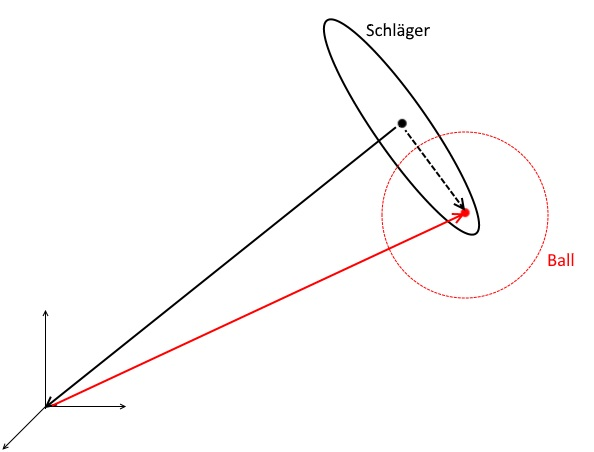
\includegraphics[scale=0.4]{bilder/collisionRacket}\label{fig_colRacket}
   \end{center} 
    \caption{Kollisionserkennung zwischen Schläger und Ball}
        \label{fig_colRacket2}
\end{figure} 

Ist eine Kollision aufgetreten, so kann der Ball entsprechend der Formel \ref{reflexion}) reflektiert werden.

\begin{equation}	
\label{reflexion}
	\vec{v}_{neu} = 2* \langle \vec{n},\vec{-v} \rangle * \vec{n} + \vec{v}
\end{equation}

Um den neuen Vektor zu berechnen muss zunächst der Einfallsvektor des Balls auf den Normalenvektor projiziert werden (gesucht ist also eine Faktor $k$, sodass $k\vec{n}$ eine Projektion von $-\vec{v}$ nach $\vec{n}$ ist). Der Einfallsvektor wird deswegen invertiert, weil ein Ausfallsvektor gesucht wird, der nicht wie der Einfallsvektor in Richtung der Ebene zeigt. $k$ lässt sich mithilfe des Skalarprodukts $\langle\vec{n},-\vec{v}\rangle$ berechnen, da der Normalenvektor einer Ebene in unserer Implementierung immer normiert gespeichert wird.



    \begin{figure}
	\begin{center}
    \subfigure[Projektion des Einfallsvektors auf den Normalvektor]
          {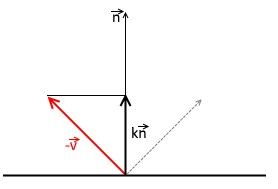
\includegraphics[scale=0.8]{bilder/reflexion1}\label{fig_reflexion_a}
    }
    \hspace{1.5cm}%
    \subfigure[Zusammensetzung des Ausfallsvektors]
         {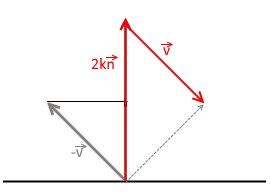
\includegraphics[scale=0.8]{bilder/reflexion2}\label{fig_reflexion_b}
             \label{abb2}

    }
    \caption{Berechnung des neuen Vektors bei einer Reflexion an einer Ebene mit Normalenvektor}
        \label{fig_reflexion}
	\end{center}
    \end{figure}
    
Die Länge des Projizierten Vektors $k\vec{n}$ muss nun, wie in Abbildung \ref{abb2} zu sehen, verdoppelt werden und zum Einfallsvektors $\vec{v}$ addiert werden. Das Ergebnis ist dann der Ausfallwinkel in entsprechender Richtung. Soll der Ausfallsvektor betragsmäßig kleiner sein (d.h. der Ball soll z.B. beim Abprallen an Wänden an Geschwindigkeit verlieren), kann der Vorfaktor 2 entsprechend verringert werden (In unserer Implementierung beträgt der Wert: 1,75).